\chapter{Entalpias de reação}\label{ch:b2:reaction-enthalpy}

Um cartucho de gás de camping rosqueado sob um pequeno fogareiro: alguns
gramas de butano levam um litro de água à fervura em poucos minutos, e a
chama azul sob a panela é muito mais quente do que a água que ferve.
Quanto calor uma reação libera, quanto dele chega à panela, e até que
temperatura a chama pode chegar? Nenhuma dessas perguntas precisa de um
fogareiro para ser respondida: tabelas com alguns números por substância,
medidos de uma vez por todas, dão o calor de toda reação que se pode
escrever com essas substâncias, a qualquer temperatura. Este capítulo
monta essa contabilidade. Ele aplica a primeira lei da termodinâmica,
conhecida da física, a um sistema cuja composição muda, define a entalpia
de uma reação como uma derivada parcial e mostra como calculá-la a partir
das entalpias de formação, das entalpias de ligação e ao longo de ciclos,
como ela varia com a temperatura e o que ela diz sobre chamas e
calorímetros.

\begin{recall}
Da física: a primeira lei $\Delta U = W + Q$; a entalpia $H = U + pV$,
uma função de estado; a pressão externa constante, entre dois estados a
essa pressão, o calor recebido é $Q_p = \Delta H$; a capacidade calorífica
a pressão constante $C_p = (\partial H/\partial T)_p$; a entalpia de um
gás perfeito depende apenas de $T$. O volume do 1.º ano descreveu um
sistema em reação por seu avanço $\xi$ e pelos números estequiométricos
$\nu_i$ de
$0 = \sum_i\nu_i\mathrm A_i$, e fixou o estado padrão de cada espécie
em $p^\circ = \qty{1}{bar}$. O volume escolar (ano 11) chamou uma reação de
\omterm{def:b2:reaction-enthalpy:exothermic}{exotérmica} quando ela libera calor e estimou energias de combustão a partir
de energias de ligação.
\end{recall}

\begin{omfigure}
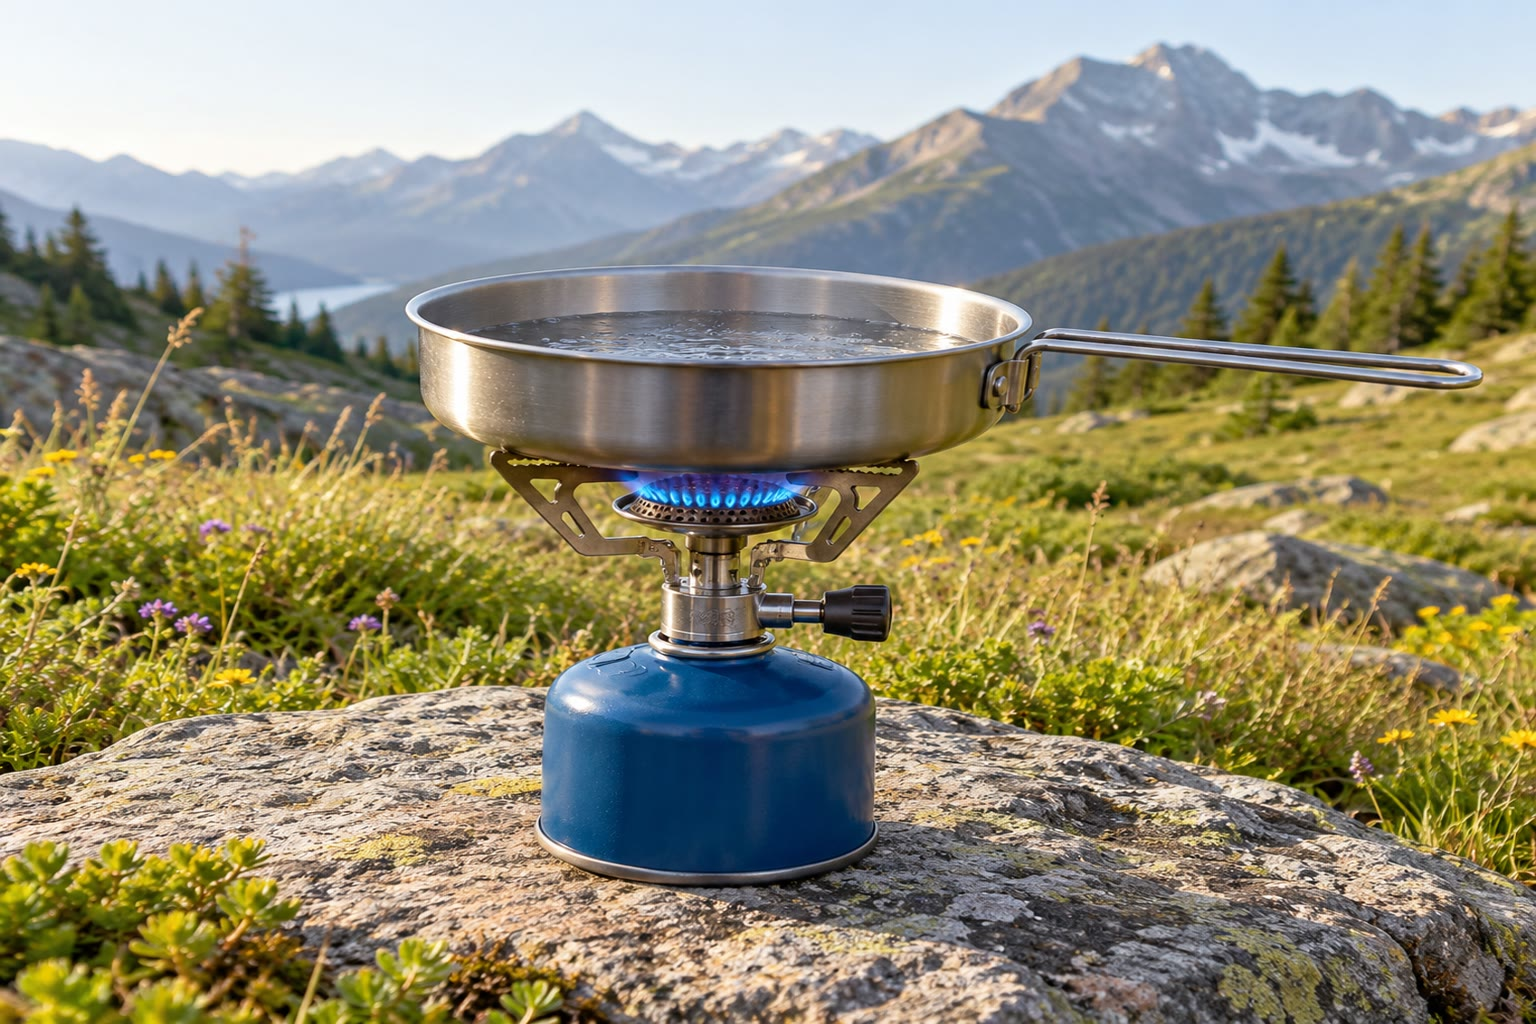
\includegraphics[width=0.6\linewidth]{images/book3/ai/b2-01-camping-stove.jpg}

{\small Um fogareiro de camping: o butano do cartucho queima no ar sob a
panela. O calor liberado por mol de butano, a parte que chega à água e a
temperatura da chama são calculados no problema de fim de semana deste
capítulo.}
\end{omfigure}

\section{Grandezas de reação}

Um sistema fechado no qual ocorre a única reação $0 = \sum_i\nu_i\mathrm A_i$
é descrito por sua temperatura, sua pressão e seu avanço: as quantidades
são $n_i = n_{i,0} + \nu_i\xi$. Toda função de estado extensiva do
sistema, sua entalpia por exemplo, é então uma função $H(T, p,
\xi)$, e sua diferencial exata é
\[
  \dd H = \left(\frac{\partial H}{\partial T}\right)_{p,\xi}\dd T
        + \left(\frac{\partial H}{\partial p}\right)_{T,\xi}\dd p
        + \left(\frac{\partial H}{\partial \xi}\right)_{T,p}\dd\xi .
\]

\begin{definition}[Grandeza de reação, entalpia de reação]\label{def:b2:reaction-enthalpy:reaction-quantity}
Para uma função de estado extensiva $X$ de um sistema fechado no qual
ocorre a reação $0 = \sum_i\nu_i\mathrm A_i$, a \emph{grandeza de
reação}\index{grandeza de reacao@grandeza de reação} é a derivada parcial
\[
  \Delta_r X = \left(\frac{\partial X}{\partial \xi}\right)_{T,p} ,
\]
a variação de $X$ por unidade de avanço a temperatura e pressão fixas, em
unidades de $X$ por mol. Para $X = H$, é a \emph{entalpia de
reação}\index{entalpia de reacao@entalpia de reação} $\Delta_r H$, em \unit{kJ/mol}.
\end{definition}

\begin{remark}[Uma derivada, não uma diferença]\label{rem:b2:reaction-enthalpy:operator}
O símbolo $\Delta_r$ é um operador: ele se aplica ao estado do
sistema, que deixa inalterado. Escrever a reação de outra forma
(dobrando seus coeficientes) dobra $\Delta_r H$; por isso uma \omterm{def:b2:reaction-enthalpy:reaction-quantity}{grandeza de
reação} não tem sentido sem sua equação. Quando se usam as entalpias
parciais molares
$\bar H_i = (\partial H/\partial n_i)_{T,p,n_j}$ das espécies
(\cref{ch:b2:chemical-potential}), $\Delta_r H = \sum_i\nu_i\bar H_i$, pela
regra da cadeia aplicada a $n_i = n_{i,0} + \nu_i\xi$.
\end{remark}

\begin{proposition}[Calor recebido a temperatura e pressão constantes]\label{prop:b2:reaction-enthalpy:qp}
Quando a reação avança de $\xi_1$ a $\xi_2$ em um sistema mantido a
$T$ e $p$ constantes, o sistema recebe o calor
\[
  Q_p = \int_{\xi_1}^{\xi_2}\Delta_r H\,\dd\xi = \Delta_r H\,(\xi_2 - \xi_1)
\]
quando $\Delta_r H$ não depende de $\xi$.
\end{proposition}

\begin{proof}
A $p$ constante (e, aqui, pressão externa constante), o calor recebido
é a variação de entalpia, $Q_p = \Delta H$ (física). A $T$ e $p$ fixos,
a diferencial de $H$ se reduz a $\dd H = \Delta_r H\,\dd\xi$; integrando
de $\xi_1$ a $\xi_2$, obtém-se o resultado.
\end{proof}

\begin{definition}[Exotérmica, endotérmica, atérmica]\label{def:b2:reaction-enthalpy:exothermic}
Uma reação é \emph{exotérmica}\index{exotermica@exotérmica} em um dado estado se
$\Delta_r H < 0$: conduzida no sentido direto a $T$ e $p$ constantes, ela
cede calor à vizinhança. Ela é \emph{endotérmica}\index{endotermica@endotérmica} se $\Delta_r H >
0$, e \emph{atérmica}\index{atermica@atérmica} se $\Delta_r H = 0$.
\end{definition}

O calor de uma reação não depende, em geral, da composição: para gases
perfeitos e para sólidos e líquidos puros, a entalpia de cada espécie não
depende do que a cerca, e $\Delta_r H$ fica fixado
uma vez fixado $T$.

\begin{proposition}[Sistemas ideais]\label{prop:b2:reaction-enthalpy:ideal}
Em uma mistura de gases perfeitos com fases condensadas puras, $\Delta_r H$
depende apenas da temperatura e é igual à \omterm{def:b2:reaction-enthalpy:standard-reaction-enthalpy}{entalpia padrão de reação}
$\Delta_r H^\circ(T)$ definida adiante. Para solutos em solução diluída,
a igualdade vale com boa aproximação.
\end{proposition}

\begin{proof}
Em uma mistura de gases perfeitos, cada gás se comporta como se estivesse
sozinho, com uma entalpia
$n_iH_{m,i}(T)$ que não depende de $p$ (física: a entalpia de um gás
perfeito depende apenas de $T$). Um sólido ou líquido puro tem $H = n_iH_{m,i}(T,
p)$, e $(\partial H_m/\partial p)_T = V_m(1 - \alpha T)$ vale alguns
\unit{J/(mol.bar)} para uma fase condensada, desprezível diante de \omterm{def:b2:reaction-enthalpy:reaction-quantity}{entalpias
de reação} de dezenas de \unit{kJ/mol}. Logo $H = \sum_in_iH_{m,i}(T)$, cuja
derivada em relação a $\xi$ é $\sum_i\nu_iH_{m,i}(T)$: ela depende apenas de
$T$, e seu valor é o calculado com todas as espécies em seu
estado padrão.
\end{proof}

\section{Entalpias padrão de reação e lei de Hess}

\begin{definition}[Grandeza padrão de reação]\label{def:b2:reaction-enthalpy:standard-reaction-enthalpy}
A \emph{grandeza padrão de reação}\index{grandeza padrao de reacao@grandeza padrão de reação}
$\Delta_r X^\circ(T) = \sum_i\nu_iX_{m,i}^\circ(T)$ é a \omterm{def:b2:reaction-enthalpy:reaction-quantity}{grandeza de reação}
calculada com todas as espécies em seu estado padrão à temperatura $T$,
sendo $X_{m,i}^\circ$ os valores molares padrão. Para $X = H$, é a
\emph{entalpia padrão de reação}\index{entalpia padrao de reacao@entalpia padrão de reação}
$\Delta_r H^\circ(T)$; ela depende apenas de $T$.
\end{definition}

Só diferenças de entalpia são mensuráveis; por isso se escolhe uma
referência de uma vez por todas, como se escolheu o eletrodo de hidrogênio
para os potenciais.

\begin{definition}[Estado padrão de referência, entalpia padrão de formação]\label{def:b2:reaction-enthalpy:formation}
O \emph{estado padrão de referência}\index{estado padrao de referencia@estado padrão de referência} de um
elemento à temperatura $T$ é sua forma mais estável a $T$ sob $p^\circ$:
\ce{H2}, \ce{O2}, \ce{N2} e \ce{Cl2} como gases perfeitos, o carbono como
grafita, o sódio como metal, o bromo como líquido (a \qty{298}{K}).
A \emph{entalpia padrão de formação}\index{entalpia padrao de formacao@entalpia padrão de formação}
$\Delta_f H^\circ$ de um composto é a \omterm{def:b2:reaction-enthalpy:standard-reaction-enthalpy}{entalpia padrão de reação} de sua
reação de formação, a que produz um mol do composto a partir de seus
elementos em seus estados de referência. Por construção,
$\Delta_f H^\circ = 0$ para um elemento em seu estado de referência.
\end{definition}

\begin{example}[Reações de formação]\label{ex:b2:reaction-enthalpy:formation}
A reação de formação da água é \ce{H2(g) + 1/2O2(g) -> H2O(l)}, com
$\Delta_f H^\circ = \qty{-285.83}{kJ/mol}$ a \qty{298.15}{K}; a do
metano é \ce{C(s) + 2H2(g) -> CH4(g)}, $\Delta_f H^\circ =
\qty{-74.9}{kJ/mol}$; a do monóxido de nitrogênio, \ce{1/2N2(g) + 1/2O2(g) ->
NO(g)}, $\Delta_f H^\circ = \qty{+90.3}{kJ/mol}$: um composto \omterm{def:b2:reaction-enthalpy:exothermic}{endotérmico},
que os gases quentes de um motor produzem mesmo assim. Os coeficientes
meios não são um problema: a reação de formação é um instrumento de
contabilidade, não um mecanismo.
% ledger: dfh:H2O-l, dfh:CH4_g, dfh:NO_g
\end{example}

\begin{theorem}[Lei de Hess]\label{thm:b2:reaction-enthalpy:hess}
Se uma reação é a soma, com coeficientes $\lambda_k$, de reações $k$,
sua \omterm{def:b2:reaction-enthalpy:standard-reaction-enthalpy}{entalpia padrão de reação} é a mesma combinação das entalpias delas:
$\Delta_r H^\circ = \sum_k\lambda_k\Delta_r H_k^\circ$
(\emph{lei de Hess}\index{lei de Hess}). Em particular, uma \omterm{def:b2:reaction-enthalpy:standard-reaction-enthalpy}{entalpia padrão
de reação} pode ser calculada ao longo de qualquer caminho de reações que
leve dos reagentes aos produtos.
\end{theorem}

\begin{proof}
Cada $\Delta_r H_k^\circ = \sum_i\nu_{i,k}H_{m,i}^\circ$ é linear nos
números estequiométricos. Se a reação é $\sum_k\lambda_k$ vezes as
reações $k$, seus números estequiométricos são $\nu_i = \sum_k\lambda_k
\nu_{i,k}$, e $\Delta_r H^\circ = \sum_i\nu_iH_{m,i}^\circ = \sum_k\lambda_k
\sum_i\nu_{i,k}H_{m,i}^\circ$. Por trás da álgebra está a primeira lei: $H$ é
uma função de estado, logo sua variação entre os mesmos estados inicial e
final não depende do caminho.
\end{proof}

\begin{proposition}[Entalpia de reação a partir das entalpias de formação]\label{prop:b2:reaction-enthalpy:formation-sum}
$\Delta_r H^\circ(T) = \sum_i\nu_i\,\Delta_f H_i^\circ(T)$.
\end{proposition}

\begin{proof}
Tome o caminho que decompõe os reagentes em seus elementos nos seus
estados de referência (o inverso de suas reações de formação, com os
coeficientes $-\nu_i > 0$) e depois forma os produtos a partir dos mesmos
elementos (coeficientes $\nu_i > 0$). Os elementos se cancelam porque a
equação está balanceada, e a \omterm{thm:b2:reaction-enthalpy:hess}{lei de Hess} soma as entalpias.
\end{proof}

\begin{omfigure}
\begin{tikzpicture}[font=\small, >={Stealth}, y=0.0062cm]
  \draw[->] (0,-1000) -- (0,180) node[above] {$H^\circ$ (\unit{kJ/mol})};
  \foreach \y in {0,-200,-400,-600,-800,-1000} \draw (-0.08,\y) -- (0.08,\y) node[left=4pt] {$\y$};
  % levels
  \draw[very thick] (1.0,0) -- (4.6,0) node[right] {\ce{C(s) + 2H2(g) + 2O2(g)}};
  \draw[very thick, omDef] (1.0,-74.9) -- (4.6,-74.9);
  \node[right, omDef] at (4.6,-110) {\ce{CH4(g) + 2O2(g)}};
  \draw[very thick, omThm] (1.0,-965.2) -- (4.6,-965.2) node[right] {\ce{CO2(g) + 2H2O(l)}};
  % arrows
  \draw[->, omDef, thick] (1.6,0) -- (1.6,-74.9);
  \node[omDef, anchor=south west, font=\footnotesize] at (1.1,5) {$\Delta_f H^\circ(\ce{CH4}) = -74.9$};
  \draw[->, omThm, thick] (3.9,0) -- (3.9,-965.2);
  \node[right, omThm, align=left] at (3.95,-500) {$\Delta_f H^\circ(\ce{CO2})$\\ $+ 2\Delta_f H^\circ(\ce{H2O})$\\ $= -965.2$};
  \draw[->, thick] (2.75,-74.9) -- (2.75,-965.2);
  \node[left, align=right] at (2.7,-650) {$\Delta_r H^\circ$\\ $= -890.3$};
\end{tikzpicture}

{\small Níveis de entalpia da combustão do metano a \qty{298.15}{K}.
Os elementos em seus estados de referência são o zero. O metano fica
\qty{74.9}{kJ/mol} abaixo deles, os produtos \qty{965.2}{kJ/mol} abaixo:
a entalpia de combustão é a diferença, \qty{-890.3}{kJ/mol}, qualquer
que seja o caminho realmente seguido pela chama.}
% ledger: dfh:CH4_g, dfh:CO2, dfh:H2O-l
\end{omfigure}

\begin{example}[Combustão do metano]\label{ex:b2:reaction-enthalpy:methane}
Para \ce{CH4(g) + 2O2(g) -> CO2(g) + 2H2O(l)},
$\Delta_r H^\circ = -393.51 + 2(-285.83) - (-74.87) - 0 =
\qty{-890.3}{kJ/mol}$ a \qty{298.15}{K}. O valor medido em um
calorímetro é \qty{-890.7}{kJ/mol}: a tabela e a chama concordam dentro
da incerteza dos dados. Se a água sai como vapor
($\Delta_f H^\circ = \qty{-241.83}{kJ/mol}$), $\Delta_r H^\circ =
\qty{-802.3}{kJ/mol}$: a diferença, \qty{88.0}{kJ}, é a entalpia de
vaporização de dois mols de água, que uma caldeira a gás recupera ao
condensar seus gases de combustão.
% ledger: dfh:CO2, dfh:H2O-l, dfh:CH4_g, dch:CH4, dfh:H2O_g (computed in figdata/bachelor-2/thermo-data.py)
\end{example}

\begin{method}[Um ciclo de Hess]\label{met:b2:reaction-enthalpy:hess-cycle}
Para obter a entalpia de uma reação que não pode ser medida diretamente:
\begin{enumerate}
  \item escreva a reação-alvo com os estados físicos;
  \item encontre reações de entalpia conhecida (combustões, formações) cuja
        combinação, com coeficientes $\lambda_k$, dê a reação-alvo;
  \item verifique que toda espécie que não está na reação-alvo se cancela;
  \item some as entalpias com os mesmos coeficientes.
\end{enumerate}
\end{method}

\begin{example}[Do carbono ao monóxido de carbono]\label{ex:b2:reaction-enthalpy:co}
Queimar carbono sempre produz algum dióxido de carbono; por isso a entalpia
de \ce{C(s) + 1/2O2(g) -> CO(g)} não é medida diretamente. As duas
combustões \ce{C(s) + O2(g) -> CO2(g)} ($\qty{-393.51}{kJ/mol}$) e \ce{CO(g) +
1/2O2(g) -> CO2(g)} ($\qty{-283.0}{kJ/mol}$, medida) o são; a reação-alvo
é a primeira menos a segunda: $\Delta_r H^\circ = -393.51 + 283.0 =
\qty{-110.5}{kJ/mol}$, a entalpia de formação do monóxido de carbono.
% ledger: dfh:CO2, dfh:CO_g
\end{example}

\begin{history}[Germain Henri Hess]
\begin{minipage}[t]{0.2\linewidth}\vspace{0pt}
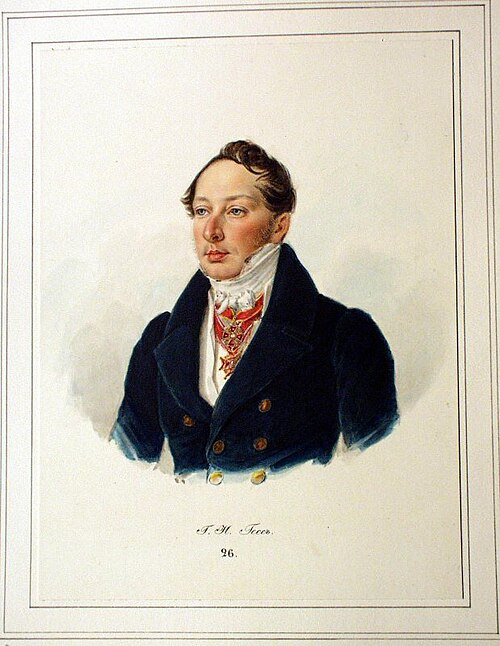
\includegraphics[width=\linewidth]{images/book3/hess.jpg}
\end{minipage}\hfill
\begin{minipage}[t]{0.76\linewidth}\vspace{0pt}
Germain Henri Hess (1802--1850), professor de química em São
Petersburgo, mediu os calores liberados quando o ácido sulfúrico é diluído
ou neutralizado em várias etapas e constatou, em 1840, que o total não
dependia das etapas seguidas: a ``lei da soma constante dos calores'',
enunciada antes da própria primeira lei da termodinâmica, que a explica.
(Retrato por I. I. Reimers, 1837--1838; CC BY-SA 4.0, Wikimedia Commons.)
\end{minipage}
\end{history}

\section{Cálculo das entalpias de reação}

\subsection*{A partir das entalpias de ligação}

Quando falta a entalpia de formação de um composto, a energia de suas
ligações dá uma estimativa, em fase gasosa.

\begin{definition}[Entalpia de dissociação de ligação, entalpia média de ligação]\label{def:b2:reaction-enthalpy:bond-enthalpy}
A \emph{entalpia de dissociação de ligação}\index{entalpia de dissociacao de ligacao@entalpia de dissociação de ligação} de
uma ligação A--B em uma molécula gasosa é a \omterm{def:b2:reaction-enthalpy:standard-reaction-enthalpy}{entalpia padrão de reação} da
ruptura dessa ligação em dois fragmentos gasosos, \ce{AB(g) -> A(g) + B(g)}
para uma molécula diatômica. Quando uma molécula tem $n$ ligações iguais, sua
\emph{entalpia média de ligação}\index{entalpia media de ligacao@entalpia média de ligação} é a entalpia
padrão de sua atomização completa em átomos gasosos dividida por $n$.
\end{definition}

As entalpias de atomização são, elas mesmas, entalpias de formação: as dos
átomos gasosos, menos a da molécula. A tabela abaixo é calculada
dessa maneira.

\begin{omfigure}
\begin{tabular}{lrl}
\hline
ligação & entalpia (\unit{kJ/mol}) & obtida de \\
\hline
H--H & 436 & \ce{H2}, dissociação \\
O=O & 498 & \ce{O2}, dissociação \\
N$\equiv$N & 945 & \ce{N2}, dissociação \\
Cl--Cl & 243 & \ce{Cl2}, dissociação \\
H--Cl & 432 & \ce{HCl}, dissociação \\
C--H & 416 & \ce{CH4}, média de quatro \\
N--H & 391 & \ce{NH3}, média de três \\
O--H & 464 & \ce{H2O}, média de duas \\
C=O & 804 & \ce{CO2}, média de duas \\
C--C & 330 & \ce{C2H6}, com C--H tomada do metano \\
C=C & 589 & \ce{C2H4}, com C--H tomada do metano \\
\hline
\end{tabular}

\smallskip
{\small Entalpias de ligação a \qty{298.15}{K}, calculadas a partir das
\omterm{def:b2:reaction-enthalpy:formation}{entalpias padrão de formação} dos átomos e das moléculas gasosos. As duas
últimas linhas mostram o limite do método: uma ligação C--H do etano não é
exatamente uma do metano, e o valor de C--C herda a diferença.}
% ledger: dfh:C_g, janaf:H, dfh:O_g, dfh:N_g, janaf:Cl, janaf:HCl, dfh:CH4_g, dfh:NH3_g, dfh:H2O_g, dfh:CO2, dfh:C2H6_g, dfh:C2H4_g (computed in figdata/bachelor-2/thermo-data.py)
\end{omfigure}

\begin{proposition}[Estimativa a partir das entalpias de ligação]\label{prop:b2:reaction-enthalpy:bond-estimate}
Para uma reação entre gases,
\[
  \Delta_r H^\circ \approx \sum(\text{entalpias das ligações rompidas}) -
  \sum(\text{entalpias das ligações formadas}).
\]
\end{proposition}

\begin{proof}
Siga o caminho que atomiza todos os reagentes (entalpia: as ligações
rompidas) e depois constrói os produtos a partir dos átomos (menos as
ligações formadas). A \omterm{thm:b2:reaction-enthalpy:hess}{lei de Hess} torna a soma exata quando cada entalpia
de ligação é a da ligação em sua própria molécula; substituí-la por um
valor médio tirado de outra molécula é a aproximação.
\end{proof}

\begin{example}[Hidrogenação do eteno]\label{ex:b2:reaction-enthalpy:hydrogenation}
Em \ce{C2H4(g) + H2(g) -> C2H6(g)}, uma C=C e uma H--H são rompidas e
substituídas por uma C--C e duas C--H. Com a tabela: $589 + 436 - 330 - 2
\times 416 = \qty{-137}{kJ/mol}$; a partir das entalpias de formação, o valor
é \qty{-136.3}{kJ/mol}. A concordância é boa aqui porque os valores de C--C
e C=C da tabela foram obtidos dessas mesmas moléculas; para uma molécula
diferente das da tabela, um erro de 10 a \qty{30}{kJ/mol} é comum.
% ledger: dfh:C2H4_g, dfh:C2H6_g
\end{example}

\subsection*{Entalpias de rede: o ciclo de Born--Haber}

\begin{definition}[Entalpia de rede]\label{def:b2:reaction-enthalpy:lattice-enthalpy}
A \emph{entalpia de rede}\index{entalpia de rede} de um cristal iônico é
a \omterm{def:b2:reaction-enthalpy:standard-reaction-enthalpy}{entalpia padrão de reação} de sua dissociação em íons gasosos: para o
cloreto de sódio, \ce{NaCl(s) -> Na+(g) + Cl-(g)}. Ela é positiva e
mede a coesão do cristal.
\end{definition}

Ela não pode ser medida diretamente, mas um ciclo pelos elementos a fornece
a partir de grandezas mensuráveis: a entalpia de formação do cristal, a
atomização dos elementos, a energia de ionização do metal e a afinidade
eletrônica do não metal (ambas definidas no volume do 1.º ano).

\begin{omfigure}
\begin{tikzpicture}[font=\small, >={Stealth}, y=0.0058cm]
  \def\lw{5.0}
  % levels (kJ/mol relative to Na(s) + 1/2 Cl2(g))
  \draw[thick] (0,0) -- (\lw,0) node[right] {\ce{Na(s) + 1/2Cl2(g)}};
  \draw[thick] (0,107.5) -- (\lw,107.5) node[right] {\ce{Na(g) + 1/2Cl2(g)}};
  \draw[thick] (0,228.8) -- (\lw,228.8) node[right] {\ce{Na(g) + Cl(g)}};
  \draw[thick] (0,724.6) -- (\lw,724.6) node[right] {\ce{Na+(g) + e- + Cl(g)}};
  \draw[thick] (0,376.1) -- (\lw,376.1) node[right] {\ce{Na+(g) + Cl-(g)}};
  \draw[thick] (0,-411.1) -- (\lw,-411.1) node[right] {\ce{NaCl(s)}};
  % the path through the elements, on the left
  \draw[->, omDef] (0.4,0) -- (0.4,107.5);
  \node[omDef, left, font=\footnotesize] at (0.35,53) {sublimação $107.5$};
  \draw[->, omDef] (0.4,107.5) -- (0.4,228.8);
  \node[omDef, left, font=\footnotesize] at (0.35,168) {$\tfrac12$ dissociação $121.3$};
  \draw[->, omDef] (0.4,228.8) -- (0.4,724.6);
  \node[omDef, left, font=\footnotesize] at (0.35,480) {ionização de Na $495.8$};
  \draw[->, omThm] (1.4,724.6) -- (1.4,376.1);
  \node[omThm, right, font=\footnotesize] at (1.45,560) {captura eletrônica $-348.6$};
  \draw[->, omProp] (2.3,0) -- (2.3,-411.1);
  \node[omProp, left, font=\footnotesize] at (2.25,-205) {formação $-411.1$};
  % the lattice enthalpy, the only unknown
  \draw[->, thick] (3.6,-411.1) -- (3.6,376.1);
  \node[right, font=\footnotesize] at (3.65,-205) {entalpia de rede $787$};
\end{tikzpicture}

{\small O ciclo de Born--Haber do cloreto de sódio a \qty{298}{K}
(\unit{kJ/mol}). Subir do cristal aos íons gasosos pela \omterm{def:b2:reaction-enthalpy:lattice-enthalpy}{entalpia de rede},
ou dar a volta pelos elementos, leva ao mesmo nível: a \omterm{def:b2:reaction-enthalpy:lattice-enthalpy}{entalpia de rede} é
a única incógnita do ciclo.}
% ledger: dfh:NaCl_cr, dfh:Na_g, janaf:Cl, ie:Na, ea:Cl
\end{omfigure}

\begin{method}[O ciclo de Born--Haber]\label{met:b2:reaction-enthalpy:born-haber}
\begin{enumerate}
  \item A partir dos elementos em seus estados de referência, trace dois
        caminhos: um até o cristal (formação), outro até os íons gasosos
        (sublimação do metal, atomização do não metal, ionização, captura
        eletrônica).
  \item Feche o ciclo com a \omterm{def:b2:reaction-enthalpy:lattice-enthalpy}{entalpia de rede}, do cristal até os íons
        gasosos.
  \item Escreva que a soma das entalpias ao longo do ciclo é nula e
        resolva para a incógnita. Energias de ionização e afinidades
        eletrônicas são tabeladas em eV por átomo: multiplique por $N_A e = \qty{96.485}{kJ/(mol.eV)}$.
\end{enumerate}
\end{method}

\begin{example}[Cloreto de sódio]\label{ex:b2:reaction-enthalpy:nacl}
$\Delta_{\text{lat}}H^\circ = 411.1 + 107.5 + 121.3 + 495.8 - 348.6 =
\qty{787}{kJ/mol}$. A energia de ionização e a afinidade eletrônica são
energias a \qty{0}{K}; suas correções para \qty{298}{K} ($+\tfrac52RT$
para cada uma) se cancelam entre as duas etapas. Um modelo de cristal com
cargas pontuais dá um valor próximo, e é por isso que o cloreto de sódio é
chamado de iônico.
% ledger: dfh:NaCl_cr, dfh:Na_g, janaf:Cl, ie:Na, ea:Cl (computed in figdata/bachelor-2/thermo-data.py)
\end{example}

\section{Entalpias de reação e temperatura}

As tabelas dão $\Delta_f H^\circ$ a \qty{298.15}{K}. Um reator opera a
\qty{700}{K}, uma chama a \qty{2000}{K}: como $\Delta_r H^\circ$ varia
com a temperatura?

\begin{theorem}[Lei de Kirchhoff]\label{thm:b2:reaction-enthalpy:kirchhoff}
\[
  \frac{\dd\Delta_r H^\circ}{\dd T} = \Delta_r C_p^\circ =
  \sum_i\nu_i C_{p,m,i}^\circ ,
\]
de modo que $\Delta_r H^\circ(T_2) = \Delta_r H^\circ(T_1) + \int_{T_1}^{T_2}
\Delta_r C_p^\circ\,\dd T$ (\emph{lei de Kirchhoff}\index{lei de Kirchhoff}),
na ausência de mudança de estado entre $T_1$ e $T_2$.
\end{theorem}

\begin{proof}
Com todas as espécies em seu estado padrão, $H^\circ(T, \xi) = \sum_in_i
H^\circ_{m,i}(T)$ é uma função de duas variáveis cujas derivadas parciais
segundas são contínuas; pelo teorema de Schwarz, elas comutam:
\[
  \frac{\dd\Delta_r H^\circ}{\dd T} = \frac{\partial}{\partial T}
  \frac{\partial H^\circ}{\partial\xi} = \frac{\partial}{\partial\xi}
  \frac{\partial H^\circ}{\partial T} = \frac{\partial}{\partial\xi}
  \sum_in_iC^\circ_{p,m,i} = \sum_i\nu_iC^\circ_{p,m,i}.
\]
Integrar entre $T_1$ e $T_2$ dá a segunda forma. Uma mudança de estado
de uma espécie dentro do intervalo acrescenta sua entalpia de transição,
multiplicada pelo número estequiométrico.
\end{proof}

\begin{example}[Síntese da amônia a quente]\label{ex:b2:reaction-enthalpy:kirchhoff}
Para \ce{N2(g) + 3H2(g) -> 2NH3(g)}, $\Delta_r H^\circ(298) =
\qty{-91.9}{kJ/mol}$ e, com as capacidades caloríficas molares a \qty{298}{K},
$\Delta_r C_p^\circ = 2(35.65) - 29.12 - 3(28.84) =
\qty{-44.3}{J/(K.mol)}$. Tomada como constante, ela dá $\Delta_r
H^\circ(700) = -91.9 - 0.0443 \times 402 = \qty{-109.7}{kJ/mol}$. As tabelas,
que acompanham o aumento das capacidades caloríficas com a temperatura, dão
\qty{-105.2}{kJ/mol}: a estimativa com $C_p$ constante erra por 4\,\%, um
preço razoável por um cálculo de uma linha. Em \qty{400}{K}, a \omterm{def:b2:reaction-enthalpy:reaction-quantity}{entalpia
de reação} varia de cerca de um sétimo.
% ledger: dfh:NH3_g, cp:NH3_g.298, cp:N2_g.298, cp:H2_g.298, janafdfH:NH3.700 (computed in figdata/bachelor-2/thermo-data.py)
\end{example}

\section{Reações adiabáticas e calorimetria}

\subsection*{Temperatura de chama}

Em uma chama, a reação é rápida e o calor não tem tempo de sair: os
gases aquecem a si mesmos.

\begin{definition}[Temperatura adiabática de chama]\label{def:b2:reaction-enthalpy:flame-temperature}
A \emph{temperatura adiabática de chama}\index{temperatura adiabatica de chama@temperatura adiabática de chama}
de um combustível é a temperatura atingida pelos produtos de sua combustão
completa quando a reação ocorre a pressão constante, sem nenhuma troca de
calor, a partir de reagentes a \qty{298}{K}.
\end{definition}

\begin{proposition}[Cálculo de uma temperatura de chama]\label{prop:b2:reaction-enthalpy:flame}
Se a reação avança de $\xi$ a partir de reagentes a $T_0$ e o sistema
final tem capacidade calorífica $C_p(T)$, a temperatura final $T_f$ satisfaz
\[
  \xi\,\Delta_r H^\circ(T_0) + \int_{T_0}^{T_f}C_p(T)\,\dd T = 0 .
\]
\end{proposition}

\begin{proof}
Adiabática e a pressão constante, a transformação tem $\Delta H =
Q_p = 0$. Como $H$ é uma função de estado, qualquer caminho entre os mesmos
estados inicial e final dá o mesmo $\Delta H$. Tome o caminho da
figura abaixo: primeiro a reação a $T_0$, com
$\Delta H_1 = \xi\Delta_r H^\circ(T_0)$ (\cref{prop:b2:reaction-enthalpy:qp},
com comportamento ideal); depois o aquecimento do sistema final de $T_0$ a
$T_f$, $\Delta H_2 = \int C_p\,\dd T$. A soma deles é nula.
\end{proof}

\begin{omfigure}
\begin{tikzpicture}[font=\small, >={Stealth}]
  \draw[->] (0,0) -- (6.2,0) node[right] {avanço $\xi$};
  \draw[->] (0,0) -- (0,3.6) node[above] {temperatura $T$};
  \fill (0.6,0.6) circle (2pt) node[below left] {reagentes, $T_0$};
  \fill (5.2,0.6) circle (2pt) node[below] {produtos, $T_0$};
  \fill (5.2,3.0) circle (2pt) node[right] {produtos, $T_f$};
  \draw[->, thick, omDef] (0.7,0.6) -- (5.1,0.6);
  \node[omDef, above, font=\footnotesize] at (3.15,0.64) {$\Delta H_1 = \xi\,\Delta_r H^\circ(T_0) < 0$};
  \draw[->, thick, omThm] (5.2,0.7) -- (5.2,2.9);
  \node[omThm, right, align=left] at (5.25,1.8) {$\Delta H_2 = \int_{T_0}^{T_f} C_p\,\dd T$};
  \draw[->, thick, dashed] (0.75,0.75) -- (5.05,2.92);
  \node[above left, align=center] at (2.6,1.75) {chama real:\\ $\Delta H = 0$};
\end{tikzpicture}

{\small A chama adiabática (tracejado) e um caminho equivalente em duas
etapas: reação a temperatura constante, depois aquecimento dos produtos.
Como $H$ é uma função de estado, as duas variações de entalpia das etapas
somam zero.}
\end{omfigure}

\begin{method}[Temperatura de chama]\label{met:b2:reaction-enthalpy:flame-temperature}
\begin{enumerate}
  \item Escreva a combustão completa de um mol de combustível; no ar,
        acrescente o nitrogênio e o argônio que acompanham o oxigênio (eles
        também são aquecidos); tome a água como vapor.
  \item Calcule $q = -\Delta_r H^\circ(T_0)$ por mol de combustível.
  \item Ou tome uma capacidade calorífica constante $C_p$ dos produtos:
        $T_f = T_0 + q/C_p$; ou encontre $T_f$ tal que a soma dos
        incrementos tabelados $n_i[H^\circ_{m,i}(T_f) - H^\circ_{m,i}(T_0)]$
        seja igual a $q$, por interpolação.
\end{enumerate}
\end{method}

\begin{omfigure}
\begin{tikzpicture}
\begin{axis}[
  width=0.8\linewidth, height=6.2cm, xmin=300, xmax=3000, ymin=0, ymax=3200,
  axis x line=bottom, axis y line=left, xlabel={$T$ (K)},
  ylabel={$H(T) - H(\qty{298}{K})$ dos produtos (kJ)},
  xtick={500,1000,1500,2000,2500,3000},
  tick label style={font=\small}, label style={font=\small}, clip=false,
  legend style={font=\scriptsize, draw=none, at={(0.5,1.03)}, anchor=south}, legend columns=2]
\addplot[omDef, very thick] table[x=T, y=H] {figdata/out/bachelor-2-flame-temperature-butane.dat};
\addplot[omThm, very thick] table[x=T, y=H] {figdata/out/bachelor-2-flame-temperature-methane.dat};
\legend{1 mol de butano no ar, 1 mol de metano no ar}
\draw[omDef, dashed] (axis cs:300,2657.6) -- (axis cs:3000,2657.6);
\node[omDef, anchor=south east, font=\scriptsize] at (axis cs:2350,2657.6) {$-\Delta_r H^\circ = \qty{2657.6}{kJ}$};
\draw[omDef, dotted] (axis cs:2401,0) -- (axis cs:2401,2657.6);
\fill[omDef] (axis cs:2401,2657.6) circle (1.5pt);
\node[omDef, anchor=north west, font=\scriptsize] at (axis cs:2420,2620) {\qty{2401}{K}};
\draw[omThm, dashed] (axis cs:300,802.3) -- (axis cs:3000,802.3);
\node[omThm, anchor=south west, font=\scriptsize] at (axis cs:320,802.3) {$-\Delta_r H^\circ = \qty{802.3}{kJ}$};
\draw[omThm, dotted] (axis cs:2329,0) -- (axis cs:2329,802.3);
\fill[omThm] (axis cs:2329,802.3) circle (1.5pt);
\node[omThm, anchor=north west, font=\scriptsize] at (axis cs:2350,760) {\qty{2329}{K}};
\end{axis}
\end{tikzpicture}

{\small Entalpia necessária para aquecer os produtos de combustão de um mol
de combustível (dióxido de carbono, vapor d'água, e o nitrogênio e o
argônio do ar) a partir de \qty{298}{K}, segundo as entalpias tabeladas.
Cada curva encontra o calor liberado pela sua combustão na \omterm{def:b2:reaction-enthalpy:flame-temperature}{temperatura
adiabática de chama}: cerca de \qty{2400}{K} para o butano, \qty{2330}{K}
para o metano.}
% ledger: janafH:CO2.2400, janafH:H2O.2400, janafH:N2.2400, janafH:Ar.2400, air:N2, air:O2, air:Ar (computed in figdata/bachelor-2/flame-temperature.py)
\end{omfigure}

As temperaturas calculadas são limites superiores. Acima de cerca de
\qty{2000}{K}, o dióxido de carbono e a água começam a se dissociar em
monóxido de carbono, hidrogênio, oxigênio e radicais; essas reações
\omterm{def:b2:reaction-enthalpy:exothermic}{endotérmicas} retomam parte do calor, e uma chama real de butano no ar é
sensivelmente mais fria do que o cálculo. No oxigênio puro, não há
nitrogênio a aquecer e a chama é muito mais quente; é por isso que os
soldadores queimam o etino com oxigênio, e não com ar.

\subsection*{Calorimetria}

\begin{proposition}[Volume constante e pressão constante]\label{prop:b2:reaction-enthalpy:bomb}
Em um recipiente fechado de aço (uma bomba calorimétrica), o calor medido é $Q_V =
\Delta U$, e, para gases perfeitos e fases condensadas,
\[
  \Delta_r H = \Delta_r U + \Delta\nu_{\text{gás}}\,RT ,
\]
em que $\Delta\nu_{\text{gás}}$ é a soma dos números estequiométricos das
espécies gasosas.
\end{proposition}

\begin{proof}
$H = U + pV$, e $\Delta_r H = \Delta_r U + \partial(pV)/\partial\xi$ a
$T$ fixo. O $pV$ das fases condensadas é desprezível e, para os
gases, $pV = n_{\text{gás}}RT$ com $n_{\text{gás}} = n_{\text{gás},0} +
\Delta\nu_{\text{gás}}\xi$, cuja derivada em relação a $\xi$ é
$\Delta\nu_{\text{gás}}RT$.
\end{proof}

\begin{omfigure}
\begin{tikzpicture}[font=\small, >={Stealth}, scale=1.0]
  % outer insulated jacket
  \draw[thick, fill=gray!8] (-2.6,-0.2) rectangle (2.6,4.4);
  \draw[thick, fill=white] (-2.3,0.1) rectangle (2.3,4.1);
  % water bath
  \fill[omDef!12] (-2.3,0.1) rectangle (2.3,3.4);
  \draw[omDef!60] (-2.3,3.4) -- (2.3,3.4);
  % bomb
  \draw[very thick, fill=gray!35] (-0.75,0.5) rectangle (0.75,2.6);
  \draw[very thick, fill=gray!55] (-0.9,2.6) rectangle (0.9,2.85);
  \draw[thick] (-0.3,1.0) -- (-0.3,1.9) (0.3,1.0) -- (0.3,1.9);
  \draw[thick, fill=orange!50] (-0.3,0.95) rectangle (0.3,1.05);
  \draw[red!70!black, thick, decorate, decoration={zigzag, amplitude=1pt, segment length=3pt}] (-0.3,1.9) -- (0.3,1.9);
  % wires
  \draw (-0.3,2.85) -- (-0.3,4.7) (0.3,2.85) -- (0.3,4.7);
  % stirrer and thermometer
  \draw[thick] (1.6,0.6) -- (1.6,4.7);
  \draw[thick, fill=gray!40] (1.35,0.55) rectangle (1.85,0.75);
  \pic[transform shape] at (-1.6,0.4) {thermometer};
  % labels
  \draw (-0.75,1.6) -- (-3.3,1.6) node[left] {bomba de aço, \ce{O2} a 30 bar};
  \draw (0,1.0) -- (-3.3,0.6) node[left] {amostra em sua cápsula};
  \draw (0,1.9) -- (-3.3,2.6) node[left] {fio de ignição};
  \draw (1.0,3.0) -- (3.3,3.0) node[right] {banho de água};
  \draw (1.6,3.9) -- (3.3,4.3) node[right] {agitador};
  \draw (-1.6,3.4) -- (-3.3,3.6) node[left] {termômetro};
  \draw (2.45,0.3) -- (3.3,0.5) node[right] {camisa isolante};
\end{tikzpicture}

{\small Uma bomba calorimétrica. A amostra queima a volume constante em
oxigênio sob pressão; o calor passa para a bomba e para a água agitada,
cuja elevação de temperatura é lida no termômetro. A capacidade calorífica
do calorímetro é determinada antes, queimando um padrão de energia conhecida.}
\end{omfigure}

\begin{method}[Calorimetria]\label{met:b2:reaction-enthalpy:calorimetry}
\begin{enumerate}
  \item Calibre: queime uma massa de um padrão de energia de combustão
        conhecida (ou forneça uma energia elétrica conhecida), leia a
        elevação de temperatura $\Delta T$ e deduza a capacidade calorífica
        $C$ do calorímetro inteiro (água e recipiente, seu ``equivalente
        em água'').
  \item Queime a amostra e leia $\Delta T'$: o calor liberado é $C\,\Delta
        T'$, logo $\Delta_r U = -C\Delta T'/\xi$ a volume constante.
  \item Corrija para $\Delta_r H$ com $\Delta\nu_{\text{gás}}RT$; em um
        calorímetro aberto (a pressão constante), $\Delta_r H = -C\Delta T'/\xi$
        diretamente.
\end{enumerate}
\end{method}

\begin{example}[Uma medida na bomba]\label{ex:b2:reaction-enthalpy:bomb}
Para a combustão do butano com água líquida, $\Delta\nu_{\text{gás}} = 4
- 1 - 6.5 = -3.5$, logo $\Delta_r U = \Delta_r H + 3.5RT = -2877.6 + 8.7 =
\qty{-2868.9}{kJ/mol}$: a correção é de alguns milésimos, maior que a
incerteza de uma boa medida na bomba; por isso nunca é omitida.
% ledger: dfh:C4H10_g, dfh:CO2, dfh:H2O-l (computed in figdata/bachelor-2/thermo-data.py)
\end{example}

\begin{history}[Bombas calorimétricas, 1881]
\begin{minipage}[t]{0.2\linewidth}\vspace{0pt}
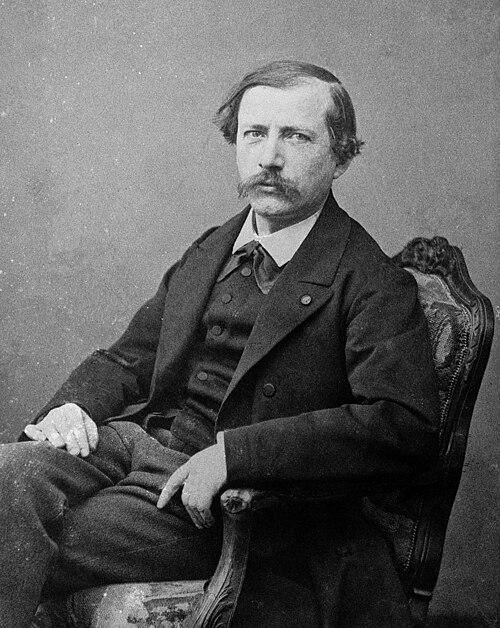
\includegraphics[width=\linewidth]{images/book3/berthelot.jpg}
\end{minipage}\hfill
\begin{minipage}[t]{0.76\linewidth}\vspace{0pt}
Marcellin Berthelot (1827--1907) queimou compostos orgânicos em oxigênio
comprimido dentro de um recipiente fechado de aço revestido de platina,
de modo que a combustão fosse completa e nada escapasse: a bomba
calorimétrica, ainda hoje o instrumento de referência para os calores de
combustão. Foi ele também quem cunhou as palavras \omterm{def:b2:reaction-enthalpy:exothermic}{exotérmico} e
\omterm{def:b2:reaction-enthalpy:exothermic}{endotérmico}. (Fotografia: domínio público, Wikimedia Commons.)
\end{minipage}
\end{history}

\section{Exercícios}

\begin{exercise}[$\star$]\label{exo:b2:reaction-enthalpy:1}
Usando as \omterm{def:b2:reaction-enthalpy:formation}{entalpias padrão de formação} do capítulo, calcule
$\Delta_r H^\circ$ a \qty{298}{K} da combustão do propano,
\ce{C3H8(g) + 5O2(g) -> 3CO2(g) + 4H2O(l)}, dado $\Delta_f
H^\circ(\ce{C3H8}, \text{g}) = \qty{-104.7}{kJ/mol}$. A reação é
\omterm{def:b2:reaction-enthalpy:exothermic}{exotérmica}?
% ledger: dfh:C3H8_g
\end{exercise}

\begin{exercise}[$\star$]\label{exo:b2:reaction-enthalpy:2}
Calcule o calor liberado pela queima de \qty{1.00}{kg} de metano (água
formada no estado líquido) e de \qty{1.00}{kg} de di-hidrogênio, \ce{H2(g) + 1/2O2(g) ->
H2O(l)}. Qual combustível dá mais calor por quilograma?
\end{exercise}

\begin{exercise}[$\star$]\label{exo:b2:reaction-enthalpy:3}
Uma bomba calorimétrica dá $\Delta_r U = \qty{-3264}{kJ/mol}$ para a
combustão do benzeno líquido, \ce{C6H6(l) + 15/2O2(g) -> 6CO2(g) + 3H2O(l)}, a
\qty{298}{K}. Calcule $\Delta_r H$.
\end{exercise}

\begin{exercise}[$\star$]\label{exo:b2:reaction-enthalpy:4}
Dados $\Delta_r H^\circ = \qty{-393.5}{kJ/mol}$ para \ce{C(s) + O2(g) ->
CO2(g)} e $\Delta_r H^\circ = \qty{-283.0}{kJ/mol}$ para \ce{CO(g) +
1/2O2(g) -> CO2(g)}, calcule a entalpia de \ce{CO2(g) + C(s) -> 2CO(g)},
a reação que ocorre no coque quente de um alto-forno.
\end{exercise}

\begin{exercise}[$\star\star$]\label{exo:b2:reaction-enthalpy:5}
Estime, com as entalpias de ligação do capítulo, a entalpia de
\ce{CH4(g) + Cl2(g) -> CH3Cl(g) + HCl(g)}, tomando \qty{350}{kJ/mol} para
C--Cl. Depois calcule a mesma grandeza a partir das entalpias de formação,
dado $\Delta_f H^\circ(\ce{CH3Cl}, \text{g}) = \qty{-83.7}{kJ/mol}$, e
comente a diferença.
% ledger: dfh:CH3Cl_g
\end{exercise}

\begin{exercise}[$\star\star$]\label{exo:b2:reaction-enthalpy:6}
A entalpia padrão de vaporização da água a \qty{298}{K} é
$\Delta_f H^\circ(\ce{H2O}, \text{g}) - \Delta_f H^\circ(\ce{H2O},
\text{l})$. Calcule-a. Com $C_{p,m}^\circ = \qty{75.35}{J/(K.mol)}$ para
o líquido e \qty{33.59}{J/(K.mol)} para o vapor, ambas tomadas como
constantes, estime-a a \qty{400}{K} (água superaquecida sob pressão)
e compare com as tabelas, que dão $\Delta_f H^\circ =
\qty{-282.59}{kJ/mol}$ para o líquido e \qty{-242.85}{kJ/mol} para o
vapor a \qty{400}{K}.
% ledger: cp:H2O_l.298, cp:H2O_g.298, janafdfH:H2O_l.400, janafdfH:H2O_g.400
\end{exercise}

\begin{exercise}[$\star\star$]\label{exo:b2:reaction-enthalpy:7}
Use um ciclo de Born--Haber para calcular a \omterm{def:b2:reaction-enthalpy:lattice-enthalpy}{entalpia de rede} do cloreto de
potássio a partir de: $\Delta_f H^\circ(\ce{KCl}, \text{s}) = \qty{-436.7}{kJ/mol}$,
sublimação do potássio \qty{89.0}{kJ/mol}, energia de ionização do
potássio \qty{4.341}{eV}, $\Delta_f H^\circ(\ce{Cl}, \text{g}) =
\qty{121.3}{kJ/mol}$, afinidade eletrônica do cloro \qty{3.613}{eV}. Por que
ela é menor que a do cloreto de sódio?
% ledger: dfh:KCl_cr, dfh:K_g, ie:K, janaf:Cl, ea:Cl
\end{exercise}

\begin{exercise}[$\star\star$]\label{exo:b2:reaction-enthalpy:8}
Um calorímetro de copo de café é calibrado fornecendo-lhe \qty{2.00}{kJ} de
energia elétrica, o que eleva sua temperatura de \qty{0.418}{K}. Em seguida,
\qty{50.0}{mL} de ácido clorídrico a \qty{1.00}{mol/L} são misturados nele
com \qty{50.0}{mL} de solução de hidróxido de sódio a \qty{1.10}{mol/L},
ambos à mesma temperatura inicial: a temperatura sobe
\qty{0.583}{K}. Calcule a entalpia de \ce{H3O+(aq) + OH-(aq) ->
2H2O(l)}.
\end{exercise}

\begin{exercise}[$\star\star$]\label{exo:b2:reaction-enthalpy:9}
O octano, um modelo da gasolina, tem $\Delta_f H^\circ(\text{l}) =
\qty{-250.3}{kJ/mol}$. Calcule a entalpia de sua combustão (água
líquida), o calor liberado por quilograma e a massa de dióxido de carbono
emitida por megajoule. Compare com o metano.
% ledger: dfh:C8H18
\end{exercise}

\begin{exercise}[$\star\star\star$]\label{exo:b2:reaction-enthalpy:10}
Calcule a \omterm{def:b2:reaction-enthalpy:flame-temperature}{temperatura adiabática de chama} do metano queimando na
quantidade estequiométrica de oxigênio puro, com capacidades caloríficas
constantes (as do capítulo a \qty{298}{K}: \ce{CO2} 37.13, \ce{H2O(g)}
\qty{33.59}{J/(K.mol)}). Compare com o resultado no ar,
\qty{2780}{K} na mesma aproximação. Por que a chama real no oxigênio é
muito mais fria do que diz esse cálculo?
% ledger: cp:CO2_g.298, cp:H2O_g.298
\end{exercise}

\begin{exercise}[$\star\star\star$]\label{exo:b2:reaction-enthalpy:11}
A capacidade calorífica de um gás é frequentemente escrita $C_{p,m}^\circ = a + bT$. Para
a síntese da amônia, tome $\Delta_r a = \qty{-60.5}{J/(K.mol)}$ e
$\Delta_r b = \qty{0.0540}{J/(K^2.mol)}$ (ajustados às tabelas entre
\qty{300}{K} e \qty{800}{K}). Integre a \omterm{thm:b2:reaction-enthalpy:kirchhoff}{lei de Kirchhoff} de
\qty{298}{K} a \qty{700}{K} e compare com o valor das tabelas,
\qty{-105.2}{kJ/mol}, e com a estimativa com $C_p$ constante.
\end{exercise}

\begin{exercise}[$\star\star\star$]\label{exo:b2:reaction-enthalpy:12}
O monóxido de nitrogênio se forma nos motores por \ce{N2(g) + O2(g) -> 2NO(g)}.
Calcule sua \omterm{def:b2:reaction-enthalpy:standard-reaction-enthalpy}{entalpia padrão de reação} a \qty{298}{K}. Mostre que, se
$\Delta_r C_p^\circ$ é pequeno, a reação absorve aproximadamente o mesmo
calor a \qty{2000}{K}; usando as capacidades caloríficas das tabelas a
\qty{298}{K} (\ce{NO} \qty{29.85}{J/(K.mol)}, \ce{N2} 29.12, \ce{O2}
\qty{29.38}{J/(K.mol)}), estime a variação entre
\qty{298}{K} e \qty{2000}{K}. Explique por que uma reação \omterm{def:b2:reaction-enthalpy:exothermic}{endotérmica} pode
ser um problema justamente nas chamas mais quentes.
% ledger: dfh:NO_g, cp:NO_g.298, cp:N2_g.298, cp:O2_g.298
\end{exercise}

\section{Problema: O cartucho de gás de camping}

\begin{problem}[{Problema de fim de semana --- a energia do butano, uma
medida em bomba calorimétrica, a água aquecida em uma panela e a
temperatura da chama}]
\label{pb:b2:reaction-enthalpy:1}
Um fogareiro de camping queima o butano de um cartucho que contém \qty{230}{g}.
Dados a \qty{298}{K} ($\Delta_f H^\circ$ em \unit{kJ/mol}): \ce{C4H10(g)}
$-125.6$, \ce{CO2(g)} $-393.51$, \ce{H2O(l)} $-285.83$, \ce{H2O(g)}
$-241.83$. Massas molares: \ce{C4H10} \qty{58.12}{g/mol}, \ce{H2O}
\qty{18.02}{g/mol}. Capacidade calorífica da água líquida:
\qty{75.35}{J/(K.mol)}. Ar seco: \qty{20.95}{\percent} \ce{O2},
\qty{78.08}{\percent} \ce{N2}, \qty{0.93}{\percent} \ce{Ar} em volume. $R = \qty{8.314}{J/(K.mol)}$.
% ledger: dfh:C4H10_g, dfh:CO2, dfh:H2O-l, dfh:H2O_g, cp:H2O_l.298, air:O2, air:N2, air:Ar

\medskip
\noindent\textbf{Parte I --- O combustível.}
\begin{enumerate}
  \item Escreva a combustão completa do butano, com a água formada no
        estado líquido, para um mol de butano.
  \item Calcule sua \omterm{def:b2:reaction-enthalpy:standard-reaction-enthalpy}{entalpia padrão de reação} a \qty{298}{K}.
  \item Calcule-a de novo com a água formada como vapor e explique a
        diferença.
  \item Calcule o calor liberado por grama de butano em cada caso.
  \item Qual dos dois valores descreve um fogareiro de camping, cuja água
        deixa a chama como vapor?
  \item Que calor o cartucho inteiro pode liberar no fogareiro?
\end{enumerate}

\medskip
\noindent\textbf{Parte II --- Uma medida.}
Uma amostra de \qty{0.500}{g} de butano é queimada em uma bomba
calorimétrica cuja capacidade calorífica é \qty{10.00}{kJ/K}; a água
formada se condensa.
\begin{enumerate}[resume]
  \item Que grandeza uma bomba calorimétrica mede, e por quê?
  \item Calcule $\Delta\nu_{\text{gás}}$ da reação da questão 1.
  \item Calcule o $\Delta_r U$ esperado.
  \item Calcule a elevação de temperatura esperada do calorímetro.
  \item A elevação lida é \qty{2.461}{K}. Deduza o $\Delta_r U$ e o
        $\Delta_r H$ medidos e a diferença relativa em relação às tabelas.
\end{enumerate}

\medskip
\noindent\textbf{Parte III --- A panela.}
\begin{enumerate}[resume]
  \item Calcule o calor necessário para levar \qty{1.00}{L} de água
        (\qty{1.00}{kg}) de \qty{20}{\celsius} a \qty{100}{\celsius}.
  \item O fogareiro faz isso com \qty{16.0}{g} de butano. Calcule seu
        rendimento (calor recebido pela água sobre calor liberado).
  \item Para onde vai o resto do calor?
  \item Quantos litros de água o cartucho inteiro pode levar à fervura
        com esse rendimento?
\end{enumerate}

\medskip
\noindent\textbf{Parte IV --- A chama.}
\begin{enumerate}[resume]
  \item O butano queima na quantidade estequiométrica de ar. Calcule as
        quantidades de dinitrogênio e de argônio que acompanham o
        dioxigênio necessário a um mol de butano.
  \item Liste as quantidades dos produtos, nitrogênio e argônio incluídos.
  \item Explique, com um caminho em duas etapas, por que o calor liberado a
        \qty{298}{K} pela reação (água como vapor) é inteiramente usado para
        aquecer esses gases.
  \item Usando as capacidades caloríficas a \qty{298}{K}, \ce{CO2} 37.13,
        \ce{H2O(g)} 33.59, \ce{N2} 29.12, \ce{Ar} \qty{20.79}{J/(K.mol)},
        calcule a capacidade calorífica dos produtos.
  \item Deduza a temperatura da chama com capacidades caloríficas constantes.
  \item Os incrementos de entalpia das tabelas dão, para os produtos de um
        mol de butano, \qty{2515.7}{kJ} entre \qty{298}{K} e
        \qty{2300}{K}, e \qty{2655.7}{kJ} entre \qty{298}{K} e
        \qty{2400}{K}. Encontre a temperatura da chama por interpolação linear.
  \item Por que a primeira estimativa é alta demais?
  \item Por que a temperatura medida de uma chama de butano é ainda menor?
  \item Dê a \omterm{def:b2:reaction-enthalpy:flame-temperature}{temperatura adiabática de chama} do butano no ar.
\end{enumerate}
\end{problem}
